\documentclass[conference]{IEEEtran}
\IEEEoverridecommandlockouts
\usepackage{cite}
\usepackage{amsmath,amssymb,amsfonts}
\usepackage{graphicx}
\usepackage{booktabs}
\usepackage{textcomp}
\usepackage{xcolor}
\usepackage{url}
\usepackage{listings}
\usepackage{algorithm}
\usepackage{algpseudocode}
\usepackage{tikz}
\usetikzlibrary{positioning,arrows.meta,shapes.geometric,calc}
\lstset{basicstyle=\ttfamily\scriptsize, columns=fullflexible, keepspaces=true, frame=tb, framerule=0.4pt, aboveskip=4pt, belowskip=2pt, captionpos=b, xleftmargin=2pt, showstringspaces=false, upquote=true}

\makeatletter
\newcommand{\linebreakand}{%
  \end{@IEEEauthorhalign}
  \hfill\mbox{}\par
  \mbox{}\hfill\begin{@IEEEauthorhalign}
}
\makeatother

\begin{document}

\title{Floating on Main: Detecting Unpinned Model Dependencies in MLOps}

\author{
\IEEEauthorblockN{Aditya Vardhan Khetawat}
\IEEEauthorblockA{\textit{Dept. of Artificial Intelligence \& Machine Learning} \\
\textit{Manipal University Jaipur}\\
Jaipur, Rajasthan, India \\
aditya.23fe10cai00586@muj.manipal.edu}
\and
\IEEEauthorblockN{Rishi Sharma}
\IEEEauthorblockA{\textit{Dept. of Artificial Intelligence \& Machine Learning} \\
\textit{Manipal University Jaipur}\\
Jaipur, Rajasthan, India \\
rishi.23fe10cai00587@muj.manipal.edu}
\linebreakand
\IEEEauthorblockN{Samairaa Arora}
\IEEEauthorblockA{\textit{Dept. of Artificial Intelligence \& Machine Learning} \\
\textit{Manipal University Jaipur}\\
Jaipur, Rajasthan, India \\
samairaa.23fe10cai00439@muj.manipal.edu}
\and
\IEEEauthorblockN{Dr. Manish Rai}
\IEEEauthorblockA{\textit{Dept. of Artificial Intelligence \& Machine Learning} \\
\textit{Manipal University Jaipur}\\
Jaipur, Rajasthan, India \\
manish.rai@jaipur.manipal.edu}
}

\maketitle

\begin{abstract}
Pre-trained models (PTMs) from hubs such as Hugging Face are loaded by name at run time; unless a revision is pinned, each new environment receives whatever the owner last pushed, undermining the reproducibility that MLOps requires. We present PinCheck, a static analyzer that detects model-loading call sites across seven Hugging Face interfaces, resolves identifiers through intra-file constant propagation, and classifies revision specifications. On 2,026 candidate call sites from 60 held-out repositories, PinCheck reaches 99.8\% detection precision versus 90.2\% for a line-based pattern-matching baseline, which recovers only 8.5\% of pinned revisions and 18.6\% of hub identifiers and would underestimate the pinning rate by a factor of thirteen. Applying PinCheck to 939 actively maintained GitHub repositories (12,898 call sites in 589 projects), we find that 84.9\% of projects never specify a model revision and only 1.7\% pin an immutable commit. Of the projects that lock their library dependencies, 82.1\% leave every model floating. One in five projects executes repository code via \texttt{trust\_remote\_code} without pinning it. Pinning increases with MLOps maturity (Cochran--Armitage $z=4.24$, $p<0.001$), and automated testing and popularity remain associated with it after adjustment. We release PinCheck and propose a CI-enforced model lockfile.
\end{abstract}

\begin{IEEEkeywords}
MLOps, pre-trained models, dependency management, static analysis, reproducibility, software supply chain
\end{IEEEkeywords}

\section{Introduction}
MLOps aims to make machine learning systems versioned, testable, and reproducible across their lifecycle~\cite{kreuzberger2023, sculley2015}. For code dependencies, Python projects achieve this through version constraints and lockfiles. Pre-trained models, however, have become dependencies of a different kind~\cite{yasmin2025}. A call such as \texttt{from\_pretrained("org/model")} resolves the default branch of a Git repository on Hugging Face \emph{at download time}. Model owners routinely push weight, tokenizer, template, and configuration changes in place~\cite{ajibode2025, castano2024}, and repositories can disappear: \texttt{runwayml/stable-diffusion-v1-5} was removed, breaking downstream code~\cite{habana1305}. Unless the loader passes a \texttt{revision} (ideally a commit hash), a project with fixed code and fixed library versions can still change behavior silently (Fig.~\ref{fig:float}).

\begin{figure}[t]
\centering
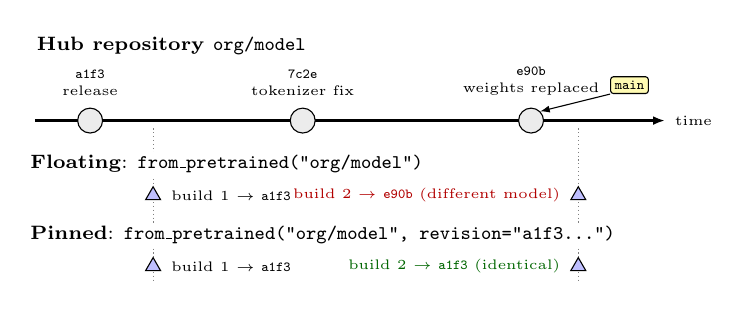
\begin{tikzpicture}[font=\scriptsize, x=1cm, y=1cm,
  cmt/.style={circle, draw, fill=gray!15, inner sep=1.3pt, minimum size=9pt},
  bl/.style={regular polygon, regular polygon sides=3, draw, fill=blue!25, inner sep=1.1pt},
  lab/.style={font=\tiny, align=center}]
% hub timeline
\node[anchor=west, font=\scriptsize\bfseries] at (-0.1,1.95) {Hub repository \texttt{org/model}};
\draw[-{Latex[length=1.5mm]}, thick] (0,1) -- (8.0,1) node[right, font=\tiny]{time};
\node[cmt] (c1) at (0.7,1) {};  \node[lab, above=1pt of c1] {\texttt{a1f3}\\release};
\node[cmt] (c2) at (3.4,1) {};  \node[lab, above=1pt of c2] {\texttt{7c2e}\\tokenizer fix};
\node[cmt] (c3) at (6.3,1) {};  \node[lab, above=1pt of c3] {\texttt{e90b}\\weights replaced};
\node[draw, rounded corners=1pt, fill=yellow!30, font=\tiny, inner sep=1.5pt] (mn) at (7.55,1.45) {\texttt{main}};
\draw[-{Latex[length=1.2mm]}] (mn.south west) -- (c3.north east);
\draw[densely dotted, gray] (1.5,0.9) -- (1.5,-1.05); \draw[densely dotted, gray] (6.9,0.9) -- (6.9,-1.05);
% floating row
\node[anchor=west, fill=white, inner sep=1pt] at (-0.1,0.45) {\textbf{Floating}: \texttt{from\_pretrained("org/model")}};
\node[bl] (f1) at (1.5,0.05) {}; \node[lab, right=1pt of f1] {build 1 $\to$ \texttt{a1f3}};
\node[bl] (f2) at (6.9,0.05) {}; \node[lab, left=1pt of f2, text=red!70!black] {build 2 $\to$ \texttt{e90b} (different model)};
% pinned row
\node[anchor=west, fill=white, inner sep=1pt] at (-0.1,-0.45) {\textbf{Pinned}: \texttt{from\_pretrained("org/model", revision="a1f3...")}};
\node[bl] (p1) at (1.5,-0.85) {}; \node[lab, right=1pt of p1] {build 1 $\to$ \texttt{a1f3}};
\node[bl] (p2) at (6.9,-0.85) {}; \node[lab, left=1pt of p2, text=green!40!black] {build 2 $\to$ \texttt{a1f3} (identical)};
\end{tikzpicture}
\caption{A floating reference resolves the default branch (\texttt{main}) at download time, so two builds of unchanged code can load different models. A pinned commit hash always resolves to the same snapshot.}
\label{fig:float}
\end{figure}

A recent manual study of 401 projects found that only 12\% specify a PTM version~\cite{yasmin2025}. Manual analysis does not scale, however, and our experiments show that the pattern-matching techniques common in repository mining misjudge this property badly. This paper makes four contributions:
\begin{enumerate}
\item \textbf{PinCheck}, an AST-based detector for PTM loads that resolves identifiers via constant propagation and classifies revisions, evaluated on a held-out sample against a pattern-matching baseline, with an ablation of constant propagation.
\item A measurement of model pinning in 939 actively maintained repositories (12,898 call sites), including per-interface rates and \emph{pinning coverage} within projects.
\item Evidence of a \emph{pinning asymmetry} between library and model dependencies, and of widespread unpinned remote code execution.
\item A multivariable analysis linking model pinning to MLOps maturity signals, and a CI-enforceable model lockfile workflow.
\end{enumerate}

\section{Related Work}
\textit{MLOps and technical debt.} Sculley et al.\ characterized ML-specific technical debt, including unstable data dependencies~\cite{sculley2015}; the ML Test Score lists reproducibility as a production-readiness criterion~\cite{breck2017}; and Kreuzberger et al.\ define versioning of code, data, and models as a core MLOps principle~\cite{kreuzberger2023}. Calefato et al.\ mined MLOps practices such as CI adoption on GitHub~\cite{calefato2022}, but did not consider PTM dependencies.

\textit{PTM reuse and evolution.} Jiang et al.\ studied reuse of Hugging Face models~\cite{jiang2023icse}, and PeaTMOSS linked GitHub projects to the PTMs they use~\cite{jiang2024peatmoss}. Yasmin et al.\ framed PTMs as ``Software Dependencies 2.0'' and reported, by manual analysis, that 12\% of 401 projects specify a model version~\cite{yasmin2025}. On the producer side, model weights change without explicit version signals~\cite{ajibode2025}, and model repositories keep evolving after release~\cite{castano2024}.

\textit{Consequences of model change.} Updates introduce ``negative flips'' even when accuracy improves~\cite{xie2021}; the behavior of LLM services drifts between versions~\cite{chen2024chatgpt}, motivating regression testing for evolving models~\cite{ma2024}. Model hubs also host malicious code~\cite{zhao2024}, which matters because \texttt{trust\_remote\_code} executes code fetched from the model repository. \textit{Dependency management and reproducibility.} Version-constraint practices~\cite{decan2021} and update lag~\cite{kula2018} are well studied in package ecosystems, where lockfiles record exact versions and releases are immutable; a model's default branch, by contrast, can be rewritten at any time. Unspecified dependencies also commonly break notebook re-execution~\cite{pimentel2019}.

\textit{Positioning.} Table~\ref{tab:prior} contrasts this work with the closest studies. We differ in providing an evaluated automated detector, call-site granularity, current data, and analyses of code--model asymmetry, remote code, and maturity that prior work does not report.

\begin{table}[t]
\centering
\caption{Comparison With Closest Prior Work}
\label{tab:prior}
\footnotesize
\setlength{\tabcolsep}{2.5pt}
\begin{tabular}{@{}lccc@{}}
\toprule
 & \cite{yasmin2025} & \cite{ajibode2025,castano2024} & \textbf{This work} \\
\midrule
Perspective & Consumer & Producer & Consumer \\
Method & Manual & Mining & Evaluated static \\
Scale & 401 projects & Hub models & 939 repos, 12.9k sites \\
Pinning measured & Project & -- & Call site + project \\
Code vs.\ model pinning & No & No & Yes \\
Remote-code exposure & No & No & Yes \\
Link to MLOps practices & No & No & Yes \\
\bottomrule
\end{tabular}
\end{table}

\section{PinCheck: Detecting Model Dependencies}
PinCheck parses each Python file and notebook (code cells, with shell and magic lines removed) into an abstract syntax tree and visits every call. A call is a \emph{model-loading site} if its callee is \texttt{from\_pretrained} (Transformers, Diffusers, PEFT), \texttt{SentenceTransformer}, \texttt{CrossEncoder}, \texttt{hf\_hub\_download}, \texttt{snapshot\_download}, LangChain's \texttt{HuggingFaceEmbeddings}, or \texttt{pipeline} when imported from Transformers. Method calls on objects that happen to be named \texttt{pipeline} are excluded.

\textit{Identifier resolution.} The identifier argument is located by position or keyword. If it is a string literal, or a name assigned exactly one string constant in the file (\emph{intra-file constant propagation}), it is classified as a \emph{hub literal} unless it is a path, a file name, or a path-prefixed concatenation, which are \emph{local} and excluded. Unresolvable expressions are \emph{indirect}; \texttt{pipeline(task)} without a model is a \emph{default pipeline}.

\textit{Revision classification.} The \texttt{revision} keyword (also inside LangChain's \texttt{model\_kwargs}) is resolved in the same way and classified as a 40-hex \emph{hash} (immutable), a \emph{named reference} such as \texttt{"main"} (mutable), \emph{configurable} (a variable), or \emph{none}. PinCheck also records whether \texttt{trust\_remote\_code=True} is set.

Algorithm~\ref{alg:pincheck} summarizes the procedure. In the algorithm, $T$ is the syntax tree of the file, $K$ maps variable names to their unique string values, $I$ indicates a Transformers \texttt{pipeline} import, $a$ and $v$ are the identifier argument and its resolved value, and $\rho$ and $w$ are the \texttt{revision} argument and its resolved value.

\begin{algorithm}[t]
\caption{PinCheck call-site classification}
\label{alg:pincheck}
\footnotesize
\begin{algorithmic}[1]
\Require source file $S$
\State $T \gets \textsc{Parse}(S)$; $K \gets$ names bound to exactly one string constant in $T$
\State $I \gets$ \textbf{true} if $T$ imports \texttt{pipeline} from \texttt{transformers}
\For{each call $n \in T$ whose callee $\in$ the seven interfaces}
  \If{callee is \texttt{pipeline} \textbf{and} ($\neg I$ \textbf{or} $n$ is a method call)} \State \textbf{continue} \EndIf
  \State $a \gets$ identifier argument (positional or keyword); $v \gets \textsc{Resolve}(a, K)$
  \If{$a$ absent \textbf{and} callee is \texttt{pipeline}} \State $id \gets$ \textsc{Default}
  \ElsIf{$v$ undefined} \State $id \gets$ \textsc{Indirect}
  \ElsIf{$v$ is a path, file name, or path prefix} \State $id \gets$ \textsc{Local} \Comment{excluded}
  \Else \State $id \gets$ \textsc{Hub}
  \EndIf
  \State $\rho \gets$ \texttt{revision} keyword (or in \texttt{model\_kwargs}); $w \gets \textsc{Resolve}(\rho, K)$
  \If{$\rho$ absent} \State $rev \gets$ \textsc{None}
  \ElsIf{$w$ matches \texttt{[0-9a-f]\{40\}}} \State $rev \gets$ \textsc{Hash}
  \ElsIf{$w$ is a literal} \State $rev \gets$ \textsc{NamedRef}
  \Else \State $rev \gets$ \textsc{Configurable}
  \EndIf
  \State \textbf{emit} $(line, callee, id, rev, \texttt{trust\_remote\_code})$
\EndFor
\end{algorithmic}
\end{algorithm}



\textit{Design rationale.} Three choices distinguish PinCheck from text search. Parsing to an AST separates executable calls from docstrings, comments, and definitions. Resolving keyword arguments on the AST finds \texttt{revision} wherever it appears in a multi-line call. Intra-file constant propagation recovers identifiers that projects keep in module-level constants, a common style for model configuration. Restricting \texttt{pipeline} to the Transformers import avoids collisions with project functions and pipeline objects. These choices keep the analysis linear in file size, and the full corpus was processed on a single CPU core with 3\,GB of memory.

\textit{Manifest analysis.} For \texttt{transformers}, \texttt{torch}, \texttt{sentence-transformers}, and \texttt{huggingface-hub}, PinCheck records the strongest declaration in any manifest (\texttt{requirements*.txt}, \texttt{pyproject.toml}, \texttt{setup.py}, \texttt{setup.cfg}, \texttt{Pipfile}, \texttt{environment.yml}) as exact, range, unpinned, or undeclared, and detects lockfiles (Poetry, uv, Pipenv, PDM), GitHub Actions workflows, test files, and Dockerfiles.

\section{Study Design}
\textit{Research questions.} \textbf{RQ1:} How accurately does PinCheck detect model loads and revisions compared with pattern matching? \textbf{RQ2:} How prevalent is model pinning? \textbf{RQ3:} Do projects that pin libraries also pin models? \textbf{RQ4:} How common are high-risk loading patterns? \textbf{RQ5:} Is pinning associated with MLOps maturity?

\begin{figure}[t]
\centering
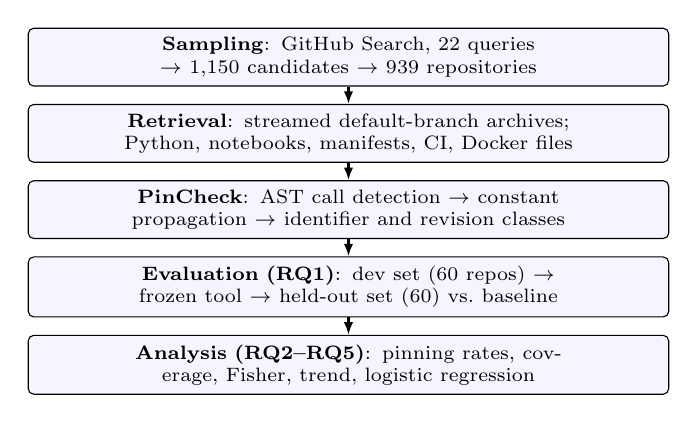
\begin{tikzpicture}[node distance=0.22cm,
  box/.style={draw, rounded corners=2pt, align=center, font=\scriptsize, text width=7.9cm, minimum height=0.5cm, fill=blue!4},
  arr/.style={-{Latex[length=1.6mm]}, thick}]
\node[box] (a) {\textbf{Sampling}: GitHub Search, 22 queries $\rightarrow$ 1,150 candidates $\rightarrow$ 939 repositories};
\node[box, below=of a] (b) {\textbf{Retrieval}: streamed default-branch archives; Python, notebooks, manifests, CI, Docker files};
\node[box, below=of b] (c) {\textbf{PinCheck}: AST call detection $\rightarrow$ constant propagation $\rightarrow$ identifier and revision classes};
\node[box, below=of c] (d) {\textbf{Evaluation (RQ1)}: dev set (60 repos) $\rightarrow$ frozen tool $\rightarrow$ held-out set (60) vs.\ baseline};
\node[box, below=of d] (e) {\textbf{Analysis (RQ2--RQ5)}: pinning rates, coverage, Fisher, trend, logistic regression};
\draw[arr] (a)--(b); \draw[arr] (b)--(c); \draw[arr] (c)--(d); \draw[arr] (d)--(e);
\end{tikzpicture}
\caption{Study pipeline, from repository sampling to the held-out detector evaluation and statistical analysis.}
\label{fig:pipeline}
\end{figure}

\textit{Sampling.} Fig.~\ref{fig:pipeline} outlines the pipeline. We queried the GitHub Search API with ten PTM-related topics (e.g., \texttt{huggingface}, \texttt{transformers}, \texttt{rag}, \texttt{semantic-search}) and twelve application keyword queries, keeping Python repositories with $\geq$20 stars, a push since 1 January 2025, and no fork or archive flag. Removing repositories over 80\,MB and the producers of the loading libraries left 939 repositories. Default-branch archives were analyzed on 20 October 2026 (one repository had been deleted); vendored library copies and virtual environments were excluded. In total, 138,940 Python files and 970 notebooks were parsed.

\textit{Metrics.} Let $C$ be a set of model-loading call sites and, for a site $c \in C$, let $r(c)$ be its \texttt{revision} argument, with $r(c)=\varnothing$ when no revision is given. The \emph{pinning rate} of $C$ is
\begin{equation}
\pi(C) = \frac{|\{c \in C : r(c) \neq \varnothing\}|}{|C|},
\label{eq:pi}
\end{equation}
where $|\cdot|$ denotes the number of elements of a set. For a repository $P$ with call sites $C_P$, we define the pinning indicator and the pinning coverage
\begin{equation}
\mathrm{pin}(P) = \begin{cases} 1 & \text{if } \pi(C_P) > 0\\ 0 & \text{otherwise,}\end{cases} \qquad \kappa(P) = \pi(C_P).
\label{eq:pin}
\end{equation}
Thus $\mathrm{pin}(P)=1$ if at least one load in $P$ specifies a revision, which gives an upper bound on pinning, and $\kappa(P)$ is the fraction of $P$'s loads that do. The \emph{strict} indicator $\mathrm{pin}^{*}(P)$ counts only sites whose $r(c)$ is a literal hash or named reference. A repository is \emph{library-pinned} if any of the four key packages is pinned with \texttt{==} or a lockfile exists. The MLOps maturity score is
\begin{equation}
M(P) = \mathbf{1}_{\mathrm{CI}}(P) + \mathbf{1}_{\mathrm{Test}}(P) + \mathbf{1}_{\mathrm{Docker}}(P) + \mathbf{1}_{\mathrm{LibPin}}(P),
\label{eq:m}
\end{equation}
where each indicator $\mathbf{1}_X(P)$ equals 1 if $P$ has property $X$ and 0 otherwise: a GitHub Actions workflow (CI), test files (Test), a Dockerfile or Compose file (Docker), and library pinning (LibPin). Hence $M(P) \in \{0,1,2,3,4\}$.

\textit{Statistics.} For a binary signal $X$, the odds ratio is
\begin{equation}
\mathrm{OR} = \frac{a/b}{c/d},
\label{eq:or}
\end{equation}
where $a$ and $b$ are the numbers of pinning and non-pinning repositories with $X$, and $c$ and $d$ those without $X$. $\mathrm{OR}>1$ means pinning is more likely when $X$ is present. Significance is assessed with two-sided Fisher exact tests, using a Bonferroni-corrected threshold of $\alpha=0.05/4=0.0125$ for the four signals. A Cochran--Armitage test checks for a linear trend in the pinning proportion across the ordered levels of $M$, and Mann--Whitney U tests compare star counts and ages. To separate correlated signals, we fit the logistic regression
\begin{equation}
\ln\frac{p_P}{1-p_P} = \beta_0 + \sum_{k=1}^{6} \beta_k x_{k}(P),
\label{eq:logit}
\end{equation}
where $p_P = \Pr(\mathrm{pin}(P)=1)$, $x_1,\dots,x_4$ are the CI, Test, Docker, and LibPin indicators, $x_5 = \log_{10}$ of the star count, and $x_6$ is the repository age in years. The adjusted odds ratio $e^{\beta_k}$ is the factor by which the odds of pinning change per unit increase in $x_k$ with the other predictors held fixed. Model fit is summarized by McFadden's
\begin{equation}
R^2_{\mathrm{McF}} = 1 - \frac{\ln \hat{L}_{\mathrm{full}}}{\ln \hat{L}_{0}},
\label{eq:r2}
\end{equation}
where $\hat{L}_{\mathrm{full}}$ and $\hat{L}_{0}$ are the maximized likelihoods of the fitted and the intercept-only models.

\textit{Detector evaluation (RQ1).} PinCheck was developed on a sample of 60 repositories (459 files). The detector was then frozen and run, together with a baseline, on a disjoint held-out sample of 60 repositories (819 files). The \emph{baseline} reflects the line-based pattern matching common in repository mining: a regular expression matches the seven callees on non-comment lines, takes the first quoted argument as the identifier, and marks a site as pinned if \texttt{revision} appears on the same line. Ground truth was built by adjudicating every disagreement between the two tools. For each task we report
\begin{equation}
\mathrm{Precision} = \frac{TP}{TP+FP}, \qquad \mathrm{Recall} = \frac{TP}{TP+FN},
\label{eq:pr}
\end{equation}
where $TP$ counts correctly reported items (call sites, hub literals, or pinned revisions), $FP$ counts reported items that are wrong, and $FN$ counts true items that were not reported. Disagreements were grouped by cause, and at least eight randomly drawn cases per cause (all cases for causes with fewer than eight) were inspected manually (definition matches were identified syntactically). In addition, 30 randomly drawn agreements were inspected; all were correct.

\section{Results}

\subsection{RQ1: Detector Accuracy}
Table~\ref{tab:eval} summarizes the held-out evaluation over 2,026 candidate sites. The baseline produced 198 false detections: 117 matches inside docstrings and documentation strings (all non-executable in the held-out set), 74 function definitions such as \texttt{def from\_pretrained(}, 3 other non-call matches (messages and a class definition), 1 invocation of a pipeline object, and 3 calls to a project-defined \texttt{pipeline} function. PinCheck's only errors were the last 3, caused by a name collision with the Transformers \texttt{pipeline}. We corrected this after the evaluation by requiring an import from Transformers, and the corrected version was used for RQ2--RQ5.

\begin{table}[t]
\centering
\caption{Held-Out Detector Evaluation (60 Repositories)}
\label{tab:eval}
\footnotesize
\setlength{\tabcolsep}{3pt}
\begin{tabular}{@{}lccc@{}}
\toprule
\textbf{Measure} & \textbf{Baseline} & \textbf{PinCheck w/o CP} & \textbf{PinCheck} \\
\midrule
Detection precision & 90.2\% & 99.8\% & 99.8\% \\
Detection recall$^{\dagger}$ & 100\% & 100\% & 100\% \\
Hub-literal recall (436) & 18.6\% & 30.3\% & 100\% \\
Hub-literal precision & 45.3\% & 100\% & 100\% \\
Revision recall (94) & 8.5\% & 100\% & 100\% \\
Estimated pinning rate & 0.4\% & 5.2\% & 5.2\% \\
\bottomrule
\multicolumn{4}{@{}p{0.95\columnwidth}@{}}{\scriptsize $^{\dagger}$Relative to the union of both tools' detections; sites missed by both cannot be counted. CP = constant propagation.}
\end{tabular}
\end{table}

\begin{table}[t]
\centering
\caption{Causes of Baseline Errors on the Held-Out Sample}
\label{tab:causes}
\footnotesize
\setlength{\tabcolsep}{3pt}
\begin{tabular}{@{}lrl@{}}
\toprule
\textbf{Cause} & \textbf{Sites} & \textbf{Effect on baseline} \\
\midrule
Identifier via constant & 304 & Hub literal missed \\
\texttt{revision} on later line & 86 & Pinning missed \\
Identifier on later line & 51 & Hub literal missed \\
Match inside docstring / string & 117 & False site \\
Function definition & 74 & False site \\
Object invocation, message, class & 4 & False site \\
Project-defined \texttt{pipeline} & 3 & False site (both tools) \\
\bottomrule
\end{tabular}
\end{table}

The baseline's deeper failure is classification. It finds only 8 of the 94 pinned revisions, because 86 appear on a later line of a multi-line call, and only 81 of the 436 hub literals, because 304 are reached through constants (\texttt{MODEL\_ID = "\ldots"}) and 51 sit on a following line. Its own hub-literal matches are mostly documentation examples (98 of 179). Consequently, the baseline would estimate the call-level pinning rate $\pi$ in (\ref{eq:pi}) at 0.4\% instead of 5.2\%, an underestimation factor of $5.2/0.4 \approx 13$. Without constant propagation, PinCheck recovers only 30.3\% of hub literals, showing that constant resolution is essential for identifying which model a project loads. 

\textbf{Answer to RQ1:} Syntax-aware analysis is necessary. Pattern matching overcounts sites, misses most identifiers and revisions, and would distort prevalence estimates by an order of magnitude.

\subsection{RQ2: Prevalence of Model Pinning}
Of the 939 repositories, 589 contain at least one non-local model load (median 245 stars, range 20--75,310). They hold 12,898 call sites referencing 825 distinct hub identifiers. Of these call sites, 78.6\% use indirect identifiers, 20.6\% hub literals, and 0.7\% no identifier. Of all call sites, 91.5\% specify no revision, 7.2\% a configurable one, 0.6\% a named reference, and 0.7\% a hash. At the project level, 500 repositories (84.9\%) never specify a revision, 63 (10.7\%) have only configurable revisions, 16 (2.7\%) use a named reference, and only 10 (1.7\%) pin any load to a hash. Just 6 (1.0\%) pin every load. Of the 2,659 hub-literal sites, 95.3\% are unpinned, and only 19 of 308 repositories with hub literals (6.2\%) pin any of them. Fig.~\ref{fig:status} compares the revision status of all sites, hub-literal sites, and remote-code sites.

\begin{figure}[t]
\centering
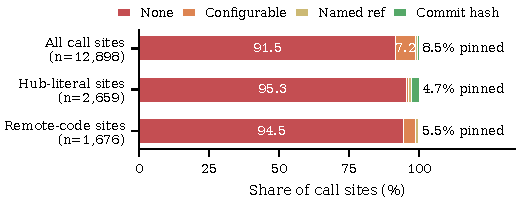
\includegraphics[width=\columnwidth]{fig_status.pdf}
\caption{Revision status of call sites (numbers inside bars are percentages). Fewer than 6\% of hub-literal and remote-code sites specify any revision, and fewer than 3\% pin a commit hash.}
\label{fig:status}
\end{figure}

Pinning depends strongly on the interface (Fig.~\ref{fig:pin}a): 32.4\% of repositories using \texttt{snapshot\_download} and 25.2\% using \texttt{hf\_hub\_download} pin at least one such call, against 12.0\% for \texttt{from\_pretrained}, 4.7\% for \texttt{SentenceTransformer}, 1.4\% for \texttt{pipeline}, and none of 26 repositories for \texttt{HuggingFaceEmbeddings}. Pinning is also partial: the median coverage among pinning repositories is 16.4\%, so a typical pinning project protects about one in six of its loads. The most common unpinned identifiers are \texttt{bert-base-uncased} (43 repositories), \texttt{all-MiniLM-L6-v2} (29), and \texttt{gpt2} (20); seven repositories still load the removed \texttt{runwayml/stable-diffusion-v1-5}.

\textit{Identifier characteristics.} Of the 308 repositories with hub literals, 52.9\% load more than one model. In 281 repositories (47.7\%) every identifier is indirect, so the loaded model cannot be determined from code. Pinning is lower in notebooks (4.4\%) than in modules (8.6\%).

\begin{figure}[t]
\centering
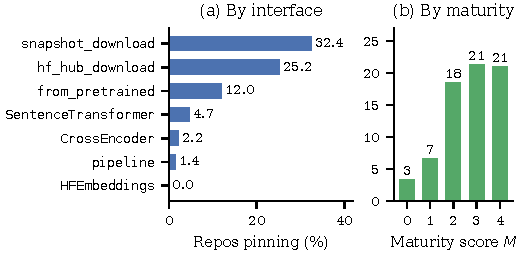
\includegraphics[width=\columnwidth]{fig_pin.pdf}
\caption{Share of repositories specifying any revision: (a) on each loading interface; (b) by MLOps maturity score $M$ ($n$ = 61, 137, 184, 131, 76).}
\label{fig:pin}
\end{figure}

\subsection{RQ3: Pinning Asymmetry}
\texttt{transformers} is pinned exactly in 21.9\% of repositories and declared with a range in 31.1\%; 21.7\% have a lockfile, and 46.5\% (274) are library-pinned overall. Of these 274 repositories, 225 (82.1\%) pin no model; the figure is 76.7\% for projects that pin \texttt{transformers} exactly and 85.2\% for projects with a lockfile. Library pinning is not significantly associated with model pinning (17.9\% vs.\ 12.7\%, OR $=1.50$, $p=0.085$). The pattern holds for every key package: \texttt{torch} is pinned exactly in 20.4\% of repositories, \texttt{huggingface-hub} in 10.5\%, and \texttt{sentence-transformers} in 7.8\%, compared with 15.1\% of repositories that specify any model revision and 1.7\% that pin a hash.



\subsection{RQ4: High-Risk Patterns}
In total, 128 repositories (21.7\%) enable \texttt{trust\_remote\_code=True} across 1,676 call sites. Of those sites, 94.5\% specify no revision and only 6 pin a hash (in 4 repositories). In 85.6\% of them the identifier is indirect, so the repository whose code is executed is chosen at run time. Almost all remote-code loads use \texttt{from\_pretrained} (1,613 sites), mostly for recent models with custom architectures. Default pipelines, whose model is chosen by the installed library version, are rare (7 repositories, 1.2\%).

\subsection{RQ5: Association With MLOps Maturity}
Pinning is more common with CI (19.4\% vs.\ 10.0\%, OR $=2.17$, $p=0.002$) and automated tests (18.2\% vs.\ 7.9\%, OR $=2.61$, $p=0.001$), both significant after correction. The association with Docker is weaker (OR $=1.67$, $p=0.029$) and does not survive correction. Pinning rises from 3.3\% at $M=0$ to 21.4\% at $M=3$ (Fig.~\ref{fig:pin}b; $z=4.24$, $p<0.001$), and pinning repositories are more popular (median 597 vs.\ 218 stars, $p<0.001$). Table~\ref{tab:logit} shows that, after adjustment, only automated tests and popularity remain significant. CI loses its effect because it is correlated with tests ($r=0.46$). Under the strict definition (26 repositories), Docker (OR $=3.35$, $p=0.005$) and library pinning (OR $=2.70$, $p=0.025$) become the strongest correlates.

\begin{table}[t]
\centering
\caption{Logistic Regression of Model Pinning ($n=589$)}
\label{tab:logit}
\footnotesize
\begin{tabular}{@{}lccc@{}}
\toprule
\textbf{Predictor} & \textbf{Adj.\ OR} & \textbf{95\% CI} & \textbf{$p$} \\
\midrule
CI workflows & 1.44 & 0.84--2.48 & 0.189 \\
Automated tests & 1.96 & 1.01--3.80 & 0.046 \\
Docker & 1.16 & 0.71--1.91 & 0.557 \\
Library-pinned & 1.43 & 0.89--2.30 & 0.140 \\
$\log_{10}$ stars & 1.52 & 1.13--2.05 & 0.005 \\
Age (years) & 0.98 & 0.88--1.10 & 0.777 \\
\midrule
\multicolumn{4}{@{}l}{LR test $p<0.001$; McFadden pseudo-$R^2=0.055$} \\
\bottomrule
\end{tabular}
\end{table}

\subsection{Robustness to Project Popularity}
For projects with at least 100, 500, and 1,000 stars ($n$ = 380, 233, 149), the share that never pin falls only to 82.1\%, 80.3\%, and 75.8\%; the asymmetry stays at 77.0--79.6\%; and 89.0--93.7\% of remote-code sites remain unpinned, while remote-code use rises from 21.7\% to 32--33\%.

\section{Discussion}


\textit{What the results mean.} Model dependencies are managed by individual choice, not project policy: coverage is low even where projects pin, and pinning concentrates in download functions that expose \texttt{revision} prominently. The asymmetry in RQ3 points to a tooling gap rather than a skills gap, since the same teams lock libraries, where lockfile tools make this automatic. In RQ5, tests and popularity, not CI by itself, distinguish pinning projects, and the low $R^2_{\mathrm{McF}}$ in (\ref{eq:r2}) shows that current practices explain little of the variation.

\textit{Why mature projects still float.} We see three plausible reasons; only the third is directly visible in our data, so developer surveys should test them. First, \emph{tooling}: a pin is a 40-character hash copied by hand from the hub, with no lockfile to generate or update it. Second, \emph{perceived stability}: popular checkpoints such as \texttt{bert-base-uncased} are widely assumed to be frozen, and updates are assumed to be improvements, so pinning looks like overhead without benefit. Third, \emph{dynamic model selection}: in 47.7\% of projects every identifier is indirect, because the model is chosen at run time through arguments or configuration. Frameworks deliberately leave this choice to users, which moves the pinning decision to whoever configures the system, where no tool checks it. Unpinned remote code is a code supply-chain risk as well as a reproducibility risk~\cite{zhao2024}.

\textit{Comparison with prior work.} Our project-level rate with any revision (15.1\%) is close to the 12\% that Yasmin et al.\ found manually~\cite{yasmin2025}, which suggests that the practice has not improved since 2023. Our strict (4.4\%) and hash-only (1.7\%) rates add that a configurable revision protects nothing unless set. Methodologically, RQ1 shows that line-based matching would have yielded a pinning rate near zero.

\textit{Recommendation: model lockfiles.} We propose committing a \texttt{models.lock} file that maps each identifier to a commit hash, loading models through a helper that reads it, and running PinCheck in CI to fail builds containing unpinned loads, unpinned remote code, or default pipelines. A model update then becomes a reviewable change that can be gated by regression tests~\cite{xie2021, ma2024} (Fig.~\ref{fig:lock}).

\begin{figure}[t]
\centering
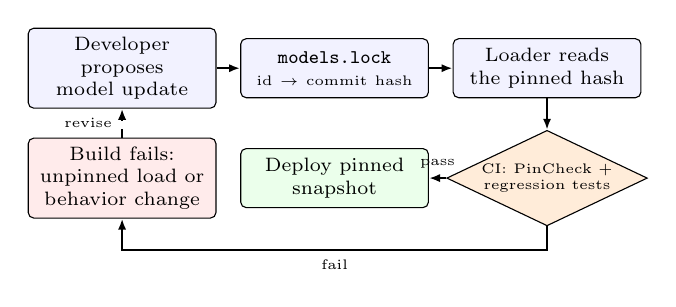
\begin{tikzpicture}[font=\scriptsize, node distance=0.35cm and 0.3cm,
  st/.style={draw, rounded corners=2pt, align=center, fill=blue!5, minimum height=0.75cm, text width=2.15cm},
  gate/.style={draw, diamond, aspect=2.1, align=center, fill=orange!15, inner sep=0.5pt, font=\tiny},
  arr/.style={-{Latex[length=1.4mm]}, thick}]
\node[st] (dev) {Developer proposes\\model update};
\node[st, right=of dev] (lock) {\texttt{models.lock}\\\tiny id $\to$ commit hash};
\node[st, right=of lock] (load) {Loader reads\\the pinned hash};
\node[gate, below=0.4cm of load] (ci) {CI: PinCheck +\\regression tests};
\node[st, fill=green!8] (dep) at (lock |- ci) {Deploy pinned\\snapshot};
\node[st, fill=red!8] (rej) at (dev |- ci) {Build fails:\\unpinned load or\\behavior change};
\draw[arr] (dev) -- (lock); \draw[arr] (lock) -- (load);
\draw[arr] (load) -- (ci);
\draw[arr] (ci.west) -- (dep.east) node[midway, above, font=\tiny] {pass};
\draw[arr] (ci.south) |- ++(0,-0.3) -| (rej.south) node[pos=0.25, below, font=\tiny] {fail};
\draw[arr, dashed] (rej.north) -- (dev.south) node[midway, left, font=\tiny] {revise};
\end{tikzpicture}
\caption{Proposed model lockfile workflow. Every load reads its commit hash from a version-controlled lockfile, and CI rejects unpinned loads, unpinned remote code, default pipelines, and behavioral regressions before deployment.}
\label{fig:lock}
\end{figure}

 \textit{Other stakeholders.} Libraries could log the resolved commit and warn on unpinned remote code, and hubs could offer immutable numbered releases.

\textit{Extending PinCheck.} Indirect identifiers usually come from three sources that a future version can resolve: \texttt{argparse} defaults and \texttt{os.getenv("KEY", default)} fallbacks in the same file; \texttt{.env} files; and YAML, JSON, or TOML configuration files such as Hydra configs. A second pass could parse these files, follow the key that the code reads (e.g., \texttt{cfg.model.name}), and report whether a matching revision key exists. Inter-procedural propagation would then cover values passed through function parameters.

\textit{Other ecosystems.} The approach generalizes because the problem does. PyTorch Hub's \texttt{torch.hub.load("owner/repo:ref")} resolves a Git branch or tag at download time, so it floats in the same way. TensorFlow Hub handles, by contrast, carry an explicit version number and are pinned by design. Hugging Face clients for JavaScript and Rust accept the same \texttt{revision} argument, so the classification rules carry over and only the parser front end must change.

\subsection{Threats to Validity}
\textit{Construct.} Indirect identifiers (78.6\% of sites) cannot be resolved statically; some are local paths or are pinned through configuration that PinCheck does not read. Configurable revisions may be unset at run time, hence the strict and hash-only rates. A few download calls fetch datasets rather than models.
\textit{Internal.} RQ5 associations are correlational, and the regression explains little variance.
\textit{External.} The sample covers public Python projects ($\geq$20 stars, active since 2025) and mixes applications with libraries, for which indirect identifiers are often intentional.
\textit{Conclusion.} Primary tests use a Bonferroni correction; strict estimates rest on 26 repositories.
\textit{Reliability.} Recall is relative to the union of both tools, and two string-embedded loads were missed during development. A re-collection on 20 October 2026 differed from one on 5 October by at most 0.2 percentage points on project-level pinning rates and 0.8 on practice signals. Only public code was analyzed, no personal data were collected, and PinCheck, the study scripts, and the datasets are publicly available at \url{https://github.com/Aditya-Khetawat/floating-on-main}.

\section{Conclusion}
We presented PinCheck and showed that syntax-aware detection is necessary to measure model dependency pinning: pattern matching would underestimate it thirteen-fold. In 589 maintained projects, model pinning is rare (84.9\% never pin; 1.7\% use hashes) and partial (median coverage 16.4\%). It is decoupled from library pinning (82.1\% asymmetry), and it is absent from most remote-code loads. Future work will measure the behavioral impact of silent updates, resolve configuration-file and environment identifiers, and extend PinCheck to PyTorch Hub and non-Python clients.

\section*{Acknowledgment}
The authors acknowledge using AI tools for paraphrasing, grammar correction, and improving readability. All research, analysis, and conclusions are the authors' own, who reviewed the revisions and remain responsible for the manuscript's accuracy and content.

\begin{thebibliography}{00}
\footnotesize
\bibitem{kreuzberger2023} D. Kreuzberger, N. K\"{u}hl, and S. Hirschl, ``Machine learning operations (MLOps): Overview, definition, and architecture,'' \emph{IEEE Access}, vol. 11, pp. 31866--31879, 2023.
\bibitem{sculley2015} D. Sculley \emph{et al.}, ``Hidden technical debt in machine learning systems,'' in \emph{Proc. NeurIPS}, 2015, pp. 2503--2511.
\bibitem{yasmin2025} J. Yasmin, W. Jiang, J. C. Davis, and Y. Tian, ``Software dependencies 2.0: An empirical study of reuse and integration of pre-trained models in open-source projects,'' arXiv:2509.06085, 2025.
\bibitem{ajibode2025} A. Ajibode, A. A. Bangash, F. R. Cogo, B. Adams, and A. E. Hassan, ``Towards semantic versioning of open pre-trained language model releases on Hugging Face,'' \emph{Empirical Software Engineering}, vol. 30, 2025.
\bibitem{castano2024} J. Casta\~{n}o, S. Mart\'{i}nez-Fern\'{a}ndez, X. Franch, and J. Bogner, ``Analyzing the evolution and maintenance of ML models on Hugging Face,'' in \emph{Proc. MSR}, 2024.
\bibitem{habana1305} ``runwayml/stable-diffusion-v1-5 no longer exists,'' Issue \#1305, huggingface/optimum-habana, GitHub, 2024. [Online]. Available: \url{https://github.com/huggingface/optimum-habana/issues/1305}
\bibitem{breck2017} E. Breck, S. Cai, E. Nielsen, M. Salib, and D. Sculley, ``The ML test score: A rubric for ML production readiness and technical debt reduction,'' in \emph{Proc. IEEE Big Data}, 2017, pp. 1123--1132.
\bibitem{calefato2022} F. Calefato, F. Lanubile, and L. Quaranta, ``A preliminary investigation of MLOps practices in GitHub,'' in \emph{Proc. ESEM}, 2022, pp. 283--288.
\bibitem{jiang2023icse} W. Jiang \emph{et al.}, ``An empirical study of pre-trained model reuse in the Hugging Face deep learning model registry,'' in \emph{Proc. ICSE}, 2023, pp. 2463--2475.
\bibitem{jiang2024peatmoss} W. Jiang \emph{et al.}, ``PeaTMOSS: A dataset and initial analysis of pre-trained models in open-source software,'' in \emph{Proc. MSR}, 2024.
\bibitem{xie2021} Y. Xie, Y.-A. Lai, Y. Xiong, Y. Zhang, and S. Soatto, ``Regression bugs are in your model! Measuring, reducing and analyzing regressions in NLP model updates,'' in \emph{Proc. ACL}, 2021, pp. 6589--6602.
\bibitem{chen2024chatgpt} L. Chen, M. Zaharia, and J. Zou, ``How is ChatGPT's behavior changing over time?'' \emph{Harvard Data Science Review}, vol. 6, no. 2, 2024.
\bibitem{ma2024} W. Ma, C. Yang, and C. K\"{a}stner, ``(Why) is my prompt getting worse? Rethinking regression testing for evolving LLM APIs,'' in \emph{Proc. CAIN}, 2024.
\bibitem{zhao2024} J. Zhao \emph{et al.}, ``Models are codes: Towards measuring malicious code poisoning attacks on pre-trained model hubs,'' in \emph{Proc. ASE}, 2024.
\bibitem{decan2021} A. Decan and T. Mens, ``What do package dependencies tell us about semantic versioning?'' \emph{IEEE Trans. Softw. Eng.}, vol. 47, no. 6, pp. 1226--1240, 2021.
\bibitem{kula2018} R. G. Kula, D. M. German, A. Ouni, T. Ishio, and K. Inoue, ``Do developers update their library dependencies?'' \emph{Empirical Software Engineering}, vol. 23, no. 1, pp. 384--417, 2018.
\bibitem{pimentel2019} J. F. Pimentel, L. Murta, V. Braganholo, and J. Freire, ``A large-scale study about quality and reproducibility of Jupyter notebooks,'' in \emph{Proc. MSR}, 2019, pp. 507--517.
\end{thebibliography}

\end{document}
